\section{Evaluation}

\subsection{Correctness and Readability}
\par According to Geuvers \cite{geuvers2009}, a proof has two major roles: 1)
to convince the readers that a statement is correct and 2) to expain
why a statement is correct. The first role requires the proof to be
convincing. The second role requires the proof to be able to give an
intuition of why the statement is correct. In the paragraphs below, we
will discuss these two criteria. 

\paragraph{Correctness} Traditionally, when a mathematician submits
the proof of his/her concepts, a group of other mathematicians will
evaluate and check the correctness of the proof. Alternatively, if we
formalise the proof in a proof assistant, the proof will be checked
automatically by the compiler. The only difference is that we are now
relying on the compiler and the machine that runs the compile rather
than the group of mathematicians. Therefore, if the compiler and the
machine works properly, then any formalised proof that
can be compiled without errors are said to be correct. In our case, we
have the type checker and the termination checker in Agda to serve the
purpose. Furthermore, a proof is consist of smaller reasoning
steps. We can say that the a proof is correct if and only if all the
reasoning steps within the proof
are correct. When writing proofs in paper, we usually omit the proofs of
some obvious lemmas and this sometime leads to mistakes. However, in
Agda, we have to provide the proofs
of every lemma we have used explicitly. Therefore, the correctness of
an Agda proof always depend on the correctness of the smaller
reasoning steps that it contains. 

\paragraph{Readability} The second purpose of a proof is to explain why
a certain statement is correct. Let us consider the following code
snippet extracted from \textbf{Correctness/RegExp-eNFA.agda}. 

\begin{center} 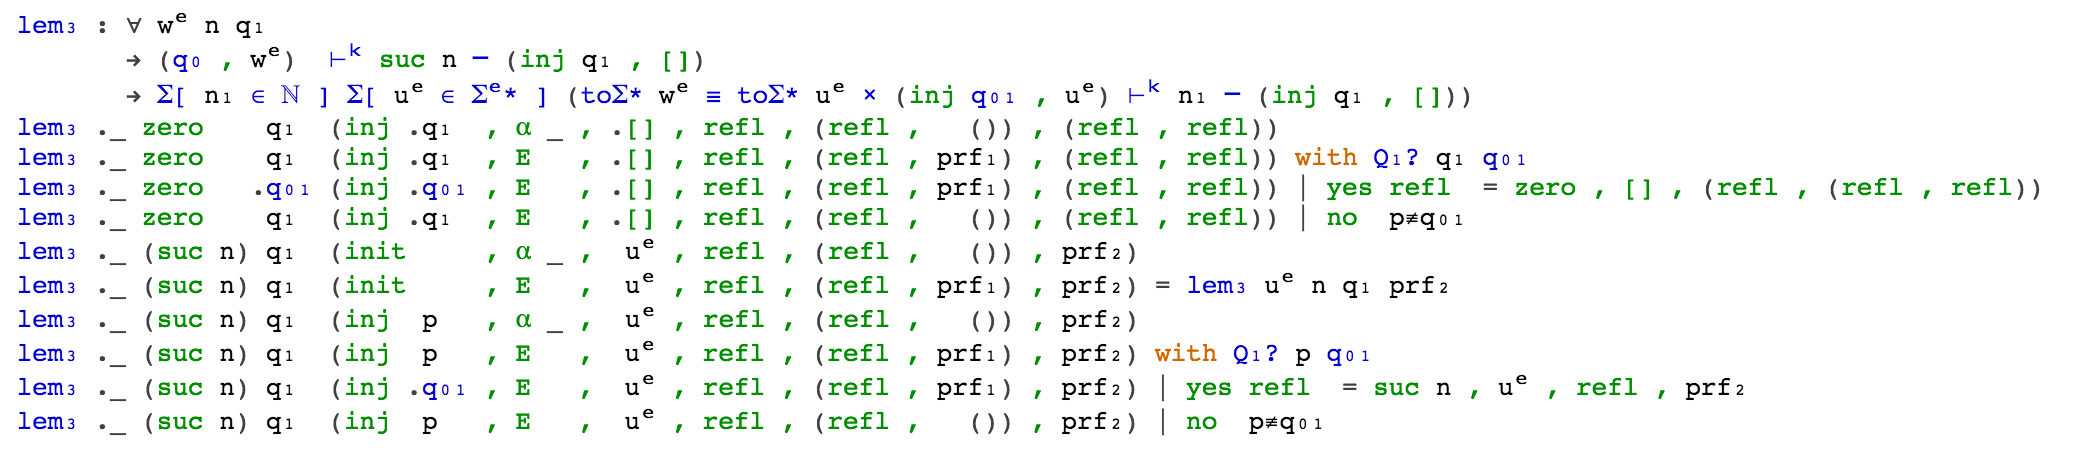
\includegraphics[width=\textwidth]{code} \end{center}

\par The above code is a proof that if \mb{w^e} can take \mb{q_0} to
another state \mb{inj\ q_1} in an \(\epsilon\)-NFA translated from a
regular expression \mb{e^*}, then there exists a number \mb{n_1} and
an \(\epsilon\)-string \mb{u^e} that will take \mb{inj\ q_{01}} to \mb{inj\ q_1} where
\mb{q_{01}} is the start state of \mb{e} and \mb{q_1} is a state in
\mb{e}. There are several techniques used in the proof including 
induction on natural numbers and case analysis of state comparison. However, by
just looking at the function body, we can hardly understand the
proving process. In conclusion, a computer proof is very inadequte on
this purpose and thus we still need to outline the concept of the proof using natural language. 


\subsection{Different choices of representations}
\par When writing computer proofs, we are usually required to
provide a concrete representation for abstract mathematical
objects. The consequence is that different represenations will lead to different
formalisations of the theorems and thus contribute to the
easiness or difficulty in completing the proofs. In our project, we have
made several decisions over the representations of different objects. In the
following parts, we will discuss their consequences. 

\paragraph{The set of states (Q) and its subsets} As we mentioned in section 3, Firsov and Uustalu
\cite{firsov2013} represented the set of states \mb{Q} and its subsets
as column matrices. However, this definition looks unnatural compare
to the actual mathematical definition. Therefore, at the beginning of
our project, we tried to avoid the vector representation. In our
apprach, the set of states are represented as a data type in Agda, i.e. \mb{Q : Set}, and its
subsets are represented as unary functions on \mb{Q}, i.e. \mb{DecSubset\ A = A \to
  Bool}. 

\par Our definiton allows us to finish the proofs in
\textbf{Correctness/RegExp-eNFA.agda} without having to
manipulate matrices. The proofs look much more natural compare to that in
\cite{firsov2013}. However, the problem arises when we need to iterate the set of states
and its subsets when we are computing the
\(\epsilon\)-closure. However, by using this definition, there is no possible way
for us to iterate the sets. Therefore, we still need to include \mb{It} -- a
vector containing all the states in \mb{Q}, in the definition of automata. By
using \mb{It}, we can iterate the subsets of \mb{Q} by applying the
function \mb{Q \to Bool} to all the elements in \mb{It}. Note that the
vector \mb{It} is actually the vector representation of the set of
states and therefore, we cannot avoid it. 

\paragraph{The language accepted by regular expression} At first, we
defined the language accepted by regular expression as a decidable
subset, i.e. \mb{L^R : RegExp \to (\Sigma^* \to Bool)}. 

\subsection{Problems arise}
\par Let us recall the definition of reachable states in
\textbf{Translation/DFA-MDFA.agda}. 

\begin{center} 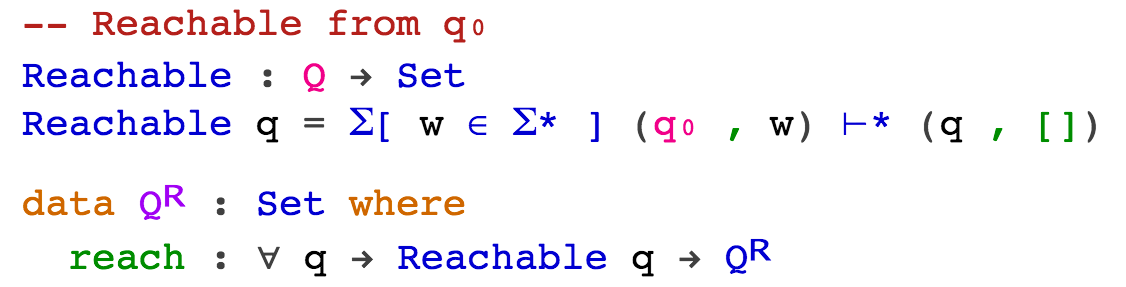
\includegraphics[width=.6\textwidth]{reach} \end{center}

\par We say that a state \mb{q} is reachable if and
only if there exists a string \mb{w} that can take \mb{q_0} to
\mb{q}. Therefore, the set \mb{Q^R} should contains all and only the
reachable states in \mb{Q}. However, there may exsist more than one
reachability proof for a single state. This implies that there may be
more than one element in \mb{Q^R} having the same state. Therefore, \mb{Q^R}
may be larger than the original set \mb{Q} or even worse, it may be
infinite. This leads to a problem when we construct a
new DFA using \mb{Q^R} as the set of states. If \mb{Q^R} is
infinite, then we have no possible way to iterate the set in 
quotient construction. Even if the set \mb{Q^R} is finite, the
computational cost will be much higher. This is also one of the
reasons why we cannot finish the quotient construction. However,
surprisingly, this has no effects to the proof of \mb{L(DFA) =
  L(MDFA)} because we can provide an equality relation of states in
the record \mb{DFA}. In the translation from DFA to MDFA, we defined
the equality relation as follow: any two states in \mb{Q^R} are equal if and only
if the input states are equal. Therefore, two elements with same state
but different reachability proofs are considered to be the same state
in the new DFA. 

\par One possible way to solve the problem is to re-define the
reachability of a state such that any reachable state will have a
unique reachability proof. For example, we can sort the reachablility
proofs according to alphabetical order of the string \mb{w} and choose the proof
with shortest string as the representative. This also requires a proof that
the chosen proof is unique. Another solution is to use
homotopy type to declare the set \mb{Q^R}. This type allows us to
group different reachability proofs into a single element such that
every state will only appear once in \mb{Q^R}. 
